\newpage
\hypertarget{sec:extendGui}{}
\section{Extending the Leitner's Box GUI}
\genHeader

\vspace{0.5cm}

In addition to \texttt{removeCard}, the GUI is able to access and operate the \texttt{check} method using your SDM implementation! To avoid build errors
however, it is currently set as a comment, so you'll need to ``activate'' it. First, double check and make sure your metamodel is built, and that you have
correctly imported the GUI.

\begin{itemize}

\item[$\blacktriangleright$] Go to ``Other Projects/LeitnersBox/Src'' and open \texttt{Leitners\-Box\-Cont\-roller\-.java} in the package.

\vspace{0.5cm}

\item[$\blacktriangleright$] On the far right side of the editor, you should be able to see two blue rectangles in the space beside the scrollbar. Click on the
second to skip ahead to the \texttt{check} invocation (Fig.~\ref{fig:remComment}).

\vspace{0.5cm}

\begin{figure}[htp]
\begin{center}
  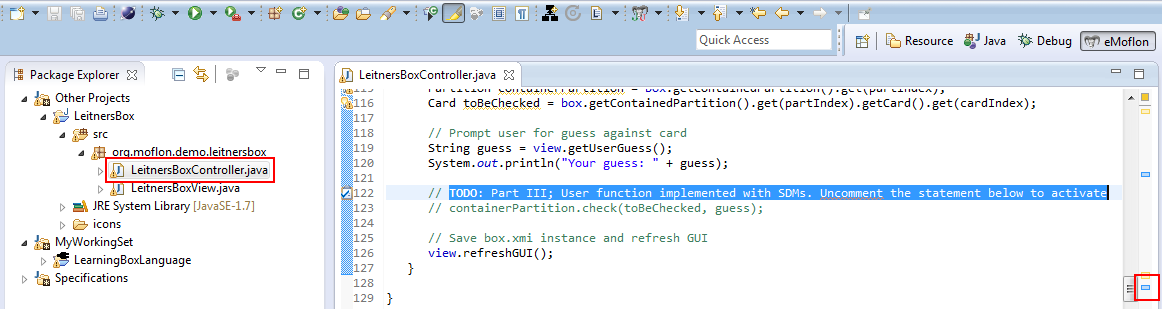
\includegraphics[width=\textwidth]{eclipse_GUICommentLine}
  \caption{Remove the comment operator on line 123}
  \label{fig:remComment}
\end{center}
\end{figure}

\vspace{0.5cm}

\item[$\blacktriangleright$] Remove the comment operators in from of the line below the \texttt{TODO} statement, save the file, then take your GUI for a spin!
Experiment with making right and wrong guesses, and watch how your cards move through the box. 

\item[$\blacktriangleright$] Keep this section in mind as you progress through the rest this part, and try extending the GUI for the remaining SDMs!

\end{itemize}
